% 原文 PDF 23--38 頁（本文 1--16 頁）、1.1--1.2。
\sectionlink{弦を概観する}\label{ch:1}
\subsectionlink{なぜ弦なのか}\label{sec:1.1}

科学の歴史における主要な主題の一つは、統一であった。多様な現象が、少数の基礎原理と構成要素によって理解されるということが、幾度となく繰り返されてきた。現在のわれわれの自然理解の基礎にある原理は、場の量子論、すなわち基本的な観測量が時空の各点に存在する量子力学である。1940年代の終わりには、場の量子論が量子力学と電磁気学を統一する正しい枠組みであることが示された。1970年代の初めまでには、弱い核力と強い核力もまた場の量子論によって記述されることが理解された。完全な理論である $SU(3)\times SU(2)\times U(1)$ 模型、すなわち標準模型は、その後、繰り返し検証されてきた。一般相対論と組み合わせると、この理論は、粒子加速器で調べられるおよそ $10^{-16}\,\mathrm{cm}$ の尺度に至るまで、事実上すべての物理と整合している。また、さらに短い距離を調べる多様な間接的検証も満たしている。これには、量子電磁力学の精密検証、稀な中間子崩壊の探索、ニュートリノ質量に対する制限、天体物理学から得られるアクシオン（軽く、弱く相互作用する粒子）に対する制限、陽子崩壊の探索、質量のないスカラーの結合に対する重力からの制限が含まれる。これらの間接的検証のいずれにおいても、新しい物理が現れても不思議ではなかったが、どの場合にも、その明確な証拠はいまだ見つかっていない。執筆時点で最も有力な兆候は、ゼロでないニュートリノ質量を示唆する太陽ニュートリノ問題である。

標準模型（および重力）は、かなり単純な構造をもつ。局所的な不変性の原理に基づく四つの相互作用がある。その一つである重力はスピン2の重力子によって媒介され、他の三つはスピン1の $SU(3)\times SU(2)\times U(1)$ ゲージボソンによって媒介される。さらに、この理論には、対称性の破れに必要なスピン0の Higgs ボソン、およびクォークとレプトンが含まれる。後者はスピン $\tfrac12$ のフェルミオンの15個の多重項であり、5個ずつ三つの世代をなす。力学は、ゲージ結合や Yukawa 結合など、およそ20個の自由パラメータに依存する Lagrangian によって支配される。

目覚ましい成功にもかかわらず、この理論が完全でないことは確かである。第一に、あまりにも恣意的である。なぜゲージ場と多重項のこの特定の構成が存在するのか、そして Lagrangian のパラメータを何が決めるのか。第二に、重力と量子論を結びつけると、繰り込み不可能な場の量子論が得られる。これは、非常に高いエネルギーで新しい物理が現れるはずだという強い兆候である。第三に、古典論の水準でさえ、一般相対論の特異点では理論が破綻する。第四に、この理論はある意味で不自然である。Lagrangian のパラメータの一部が、予想される値よりもはるかに小さいのである。より完全な理論を見いだそうとする現在の試みを導かねばならないのは、積極的な実験的証拠ではなく、これらの問題である。われわれが求めているのは、標準模型の場をより単純な構造に統一し、発散の問題と自然さの問題を解決する原理である。

いくつかの有望な考えが提案されてきた。一つは大統一である。これは三つのゲージ相互作用を一つにまとめ、各世代の五つの多重項を二つ、さらには一つにまとめる。また、自由パラメータの一つである弱混合角を正しく予言し、もう一つ、ボトムとタウの質量比をも予言する可能性がある。第二の考えは、時空には四つを超える次元があり、余分な次元は非常に強く曲がっているため、現在のエネルギーでは検出できないというものである。一般相対論では時空の幾何は力学的であるから、これは確かに論理的に可能である。この考えを魅力的にしているのは、一つの高次元の場から多数の四次元の場が生じうることである。それらは、偏極の向き（小さい次元の方向を向くことも、大きい次元の方向を向くこともある）や、小さい次元への依存性が異なる。このことは、ゲージ相互作用と重力を統一する可能性、すなわち Kaluza--Klein 機構を開く。また、同じフェルミオン多重項の反復である世代を生み出す自然な機構も与える。第三の統一原理は超対称性であり、これはスピンと統計の異なる場を関係づけ、発散と自然さの問題の解決にも役立つ。

大統一、余剰次元、超対称性というこれらの考えには、それぞれ魅力的な特徴があり、標準模型のさまざまな検証と整合している。これらが、基礎物理のより完全な理論の要素として見いだされるというのは、もっともらしい。しかし、何かがまだ欠けていることも明らかである。これらの考えを単独で、あるいは組み合わせて用いても、標準模型に比べて実質的に単純で、恣意性の少ない理論には至っていない。

短距離の発散は、場の量子論において幾度も重要な問題となってきた。たとえば、それは弱い相互作用の Fermi 理論から Weinberg--Salam 理論へ至る重要な手掛かりであった。少しの次元解析で理解できる、量子重力の短距離問題を見てみよう。図\hyperref[fig:1.1]{1.1}には、二つの粒子が伝播する過程と、1個の重力子の交換および2個の重力子の交換による補正を示している。1個の重力子の交換は Newton 定数 $G_{\mathrm N}$ に比例する。1個の重力子による補正と元の振幅との比は、無次元の組合せ $G_{\mathrm N}E^2\hbar^{-1}c^{-5}$ によって決まらねばならない。ここで $E$ はその過程の特徴的なエネルギーであり、この組合せが、問題に現れるパラメータから作ることのできる唯一の無次元量だからである。本書全体を通じて $\hbar=c=1$ となる単位を用い、Planck 質量を
\begin{equation}
M_{\mathrm P}=G_{\mathrm N}^{-1/2}=1.22\times10^{19}\,\mathrm{GeV}
\tag{1.1.1}\label{eq:1.1.1}
\end{equation}
と定義し、Planck 長さを
\begin{equation}
M_{\mathrm P}^{-1}=1.6\times10^{-33}\,\mathrm{cm}
\tag{1.1.2}\label{eq:1.1.2}
\end{equation}
と定義する。すると、重力子1個の振幅と重力子0個の振幅との比は、$(E/M_{\mathrm P})^2$ 程度となる。

\begin{figure}[htbp]
\centering
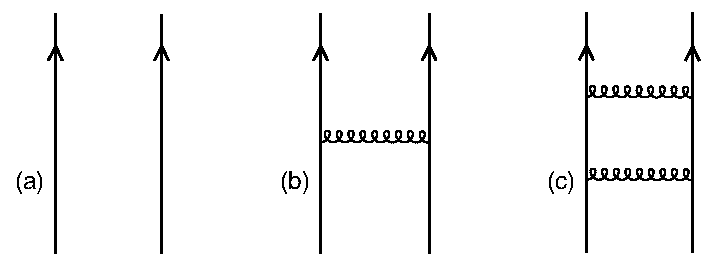
\includegraphics[width=0.8\linewidth]{figures/fig_1_1.pdf}
\caption{(a) 自由に伝播する二つの粒子。(b) 1個の重力子の交換による補正。(c) 2個の重力子の交換による補正。}
\label{fig:1.1}
\end{figure}

この次元解析から直ちに、量子重力による補正が非関連相互作用であることがわかる。これは、低エネルギーでは弱くなり、とくに数百 $\mathrm{GeV}$ という素粒子物理のエネルギーでは無視できることを意味する。同じ理由から、高エネルギーでは結合が強くなり、$E>M_{\mathrm P}$ では摂動論が破綻する。図\hyperref[fig:1.1]{1.1}(c)の重力子2個による補正では、中間状態について和をとる。エネルギーの高い $E'$ の中間状態については、次元の考察から、重力子2個の振幅と重力子0個の振幅との比は
\begin{equation}
G_{\mathrm N}^{\,2}E^2\int dE'\,E'
=\frac{E^2}{M_{\mathrm P}^{\,4}}\int dE'\,E'
\tag{1.1.3}\label{eq:1.1.3}
\end{equation}
程度となる。理論を任意に高いエネルギーまで外挿すると、これは発散する。位置空間では、この発散は、すべての重力子の頂点が一致する極限から生じる。重力子を一つ追加するごとに発散は悪化する。これが繰り込み不可能性の問題である。

考えられる解決は二つある。第一は、発散が相互作用のべきで展開することによって生じており、理論を厳密に扱えば消えるというものである。繰り込み群の言葉では、これは非自明な紫外固定点に対応する。第二は、理論を任意に高いエネルギーまで外挿することが誤りであり、あるエネルギーを超えると、時空内で相互作用を広げて発散を和らげるように理論が修正されるというものである。量子重力が非自明な紫外固定点をもつかどうかは知られていないが、第二の可能性に注目する理由はいくつもある。一つは歴史である。弱い相互作用の Fermi 理論における同種の発散問題は、新しい物理の兆候であった。フェルミオン間の接触相互作用が、より短い距離ではゲージボソンの交換として分解されたのである。もう一つは、標準模型の構成を説明するために、いずれにせよより完全な理論が必要であり、その同じ新しい物理が量子重力の発散問題も解決すると期待するのは妥当だということである。

場の量子論では、理論の整合性を保ちながら相互作用を広げることは容易でない。Lorentz 不変性が非常によい近似で成り立つことはわかっている。このことは、空間内で相互作用を広げれば時間内でも広げることになり、その結果、因果律あるいはユニタリティが失われることを意味する。さらに、Lorentz 不変性が実際には局所対称性である一般座標不変性に組み込まれていることもわかっており、これによって、不整合を生じさせずに相互作用を広げることは、いっそう難しくなる。

実際、理論の整合性を損なうことなく重力相互作用を広げ、発散を切り捨てる方法として、現在知られているものは一つしかない。それが、図\hyperref[fig:1.2]{1.2}に示す弦理論である。この理論では、重力子と他のすべての素粒子は、場の量子論のような点ではなく、一次元の物体である弦である。なぜこれがうまくいき、他のものではいけないのかは、先験的にはまったく明らかでないが、理論を展開していくにつれ、その仕組みがわかるであろう。\footnote[1]{少なくとも一つのよくある疑問、すなわちなぜ膜、つまり二次元以上の物体ではいけないのか、という疑問には直観的な答えがある。粒子をより多くの次元に広げると、時空の発散は軽減されるが、内部自由度の数の増大に由来する新しい発散に遭遇するのである。時空の発散と内部の発散の両方を制御できるのは、一次元の場合に限られるように見える。ただし、第14章で議論するように、膜という考えは、やや姿を変えて行列理論として再登場している。}
われわれには単に想像力が足りないだけであり、短距離カットオフをもつ整合的な重力理論は、ほかにも多数あるのかもしれない。しかし、場の量子論における発散問題は簡単には解決されないということを経験は示している。したがって、解決法が一つでもあるなら、それをきわめて真剣に受け止めるべきである。実際、整合性という原理がこれほど強い制約を与えることがわかったのは、幸いである。重力と他の相互作用の統一は $M_{\mathrm P}$ という非常に高いエネルギーで起こるため、実験的検証は難しく、間接的なものになるからである。

\begin{figure}[htbp]
\centering
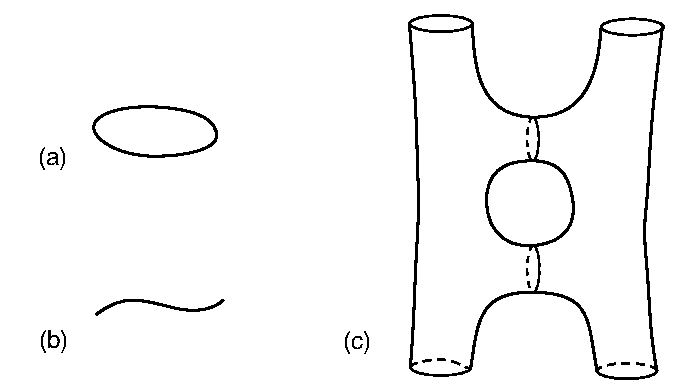
\includegraphics[width=0.8\linewidth]{figures/fig_1_2.pdf}
\caption{(a) 閉弦。(b) 開弦。(c) 弦理論における図\hyperref[fig:1.1]{1.1}(c)のループ振幅。各粒子の世界線は円筒となり、相互作用はもはや点で起こらない。（中間の線に描いた断面は、立体的な形状をわかりやすくするためだけに加えたものである。）}
\label{fig:1.2}
\end{figure}

では、この考えを追求すると何が見いだされるだろうか。一言でいえば、驚くべき結果が得られる。弦理論は、標準模型の構成を説明するための従来の考えと見事にかみ合い、しかも、場の量子論に比べていっそう優美で統一された構造のもとで、それを実現する。とくに、一次元の物体について整合的な相対論的量子論を構成しようとすると、次のことがわかる。
\begin{enumerate}
\item 重力。整合的な弦理論はすべて、質量のないスピン2の状態を含まなければならず、その相互作用は低エネルギーで一般相対論に帰着する。
\item 少なくとも摂動論の範囲では、整合的な量子重力理論。すでに述べたように、これは既知のすべての重力の場の量子論と対照的である。
\item 大統一。弦理論は、標準模型を含むのに十分大きいゲージ群を導く。最も単純な弦理論のいくつかは、標準模型の統一に現れるのと同じゲージ群とフェルミオン表現を導く。
\item 余剰次元。弦理論は、時空の次元が10という特定の数であることを要求する。\footnote[2]{正確にいうと、弦理論は時空の位相と幾何の概念を修正するので、ここで次元と呼ぶものは一般化されたものである。また、10次元は弱結合の弦理論にとって適切な数であるが、強結合では描像が変わりうることを見るであろう。}
場の方程式には、大きく平坦な四つの次元と、小さく曲がった六つの次元をもち、四次元の物理が標準模型に似ている解が存在する。
\item 超対称性。整合的な弦理論は、顕在的な対称性、または自発的に破れた対称性として、時空の超対称性を必要とする。
\item カイラルなゲージ結合。自然界のゲージ相互作用は、パリティに関して非対称、すなわちカイラルである。このことは、従来の統一の考えのいくつかにとって障害であった。それらはパリティ対称なゲージ結合を必要としていたからである。弦理論ではカイラルなゲージ結合が許される。
\item 自由パラメータがない。弦理論には調整可能な定数が存在しない。
\item 一意性。連続的なパラメータが存在しないだけでなく、場の理論におけるゲージ群や表現の選択に相当する離散的な自由も存在しない。弦理論は一意である。
\end{enumerate}
加えて、アクシオンや隠れたゲージ群など、統一の考えの中で役割を果たしてきた、ほかの多くの特徴も見いだされる。

これは、一次元の物体という単純な仮定から生じるものとして、驚くべき一覧である。最初の二項だけでも大いに興味深い。その次の四項は、標準模型を統一しようとするときに到達する描像に、驚くほど近い。そして最後の二項が示すように、弦理論は、場の量子論よりも緊密で恣意性の少ない構造によってこれを実現し、それまでの考えに欠けていた要素を与える。最初の項も、この構造の緊密さのさらなる例である。弦理論には重力子が必ず存在しなければならないのに対し、場の理論では、重力子や他の場は個別に選んで組み合わされる。

さらに、弦理論は数学の多くの分野と結びついており、それらの間に新しく予想外の関係を見いだすことにつながってきた。また、超対称な場の量子論における近年の発見と豊かな関係をもつ。弦理論は、量子重力のより深い問題の一部、とくにブラックホールの量子力学にも取り組み始めている。

もちろん、なすべきことは多く残っている。弦理論は、大筋では現実の世界に似ているかもしれないが、決定的な検証はなお遠いように思われる。主な問題は、理論は一意であるにもかかわらず、大きく平坦な四つの次元をもつ解に注意を限っても、膨大な数の古典解が存在することである。量子化すると、これらはそれぞれ理論の可能な基底状態、すなわち真空となり、各々で四次元の物理は異なる。量子効果によって安定な解の数が大きく減ることは知られているが、力学の完全な理解はいまだ得られていない。

標準模型においてさえ、真空の力学が、われわれの観測する物理で重要な役割を果たすことを思い起こしておこう。電弱相互作用では、真空の対称性が Hamiltonian の対称性より低いという事実、すなわち対称性の自発的破れが中心的な役割を果たす。強い相互作用では、真空中の大きく揺らぐゲージ場がクォークの閉じ込めをもたらす。場の量子論におけるこれらの現象は、多数の自由度をもつ量子系であることから生じる。弦理論には、はるかに多くの自由度があるように見えるため、さらに豊かな力学を期待すべきである。

さらに、「弦理論とは何か」という問題がある。つい最近まで、弦理論についてのわれわれの理解は、少数の弦が弱く相互作用する摂動論に限られていた。強結合において、理論をどのように定義すればよいのかさえ知られていなかった。弱結合で用いる自由度である一次元の物体は、究極的には、理論を理解するための最も単純で、最も完全な方法ではないのではないか、という疑いがあった。

過去数年間、これらの問題には大きな進展があった。その多くは、超対称性が課す制約を系統的に適用することから生まれた。強結合の弦の力学を完全に理解したわけでは決してないが、十分な量の超対称性が破れずに残っている場合には、真空の空間を詳細に描き出すことが可能になり、それは多くの驚きをもたらした。一つは、理論の絶対的な一意性である。弱結合の弦理論はいくつか存在するが、そのすべてが、単一の理論の真空の空間における極限であることがわかった。もう一つは、時空が11次元になる極限である。11という数は、超重力の観点からは興味深いが、弱結合の弦理論では不可能な数である。また、この理論には D-brane という新しい広がりをもつ物体が含まれることも理解され、これがブラックホールの量子力学の新しい理解につながった。これらすべては、理論の究極的な姿についても、新しく予想外の手掛かりを与えている。

まとめると、これほど多くのアプローチが、一つの有力な考えへと収束するように見えるのは幸いである。量子重力の発散問題から出発しても、標準模型の構成を説明しようとする試みから出発しても、あるいは統一理論の構成に役立ちうる新たな対称性や数学的構造の探求から出発しても、弦理論へ導かれるのである。

\subsubsectionlink*{本書の構成}

この全2巻の目標は、弦理論を初歩から始め、四次元へのコンパクト化、そして強結合の弦に関する最新の進展にまで進む、完全な入門を提供することである。

第1巻は、ボソン弦理論への入門である。これは現実的な理論ではない。フェルミオンをもたず、知られている限り、安定な基底状態ももたない。ここでの考え方は、場の量子論の講義をスカラー場の理論の徹底的な学習から始める場合と同じである。スカラー場の理論も、最終的に関心のある理論ではないが、スピンやゲージ不変性に伴う複雑さを導入する前に、場の量子論に特有の力学的・技術的な特徴を展開するための単純な例を与える。同様に、ボソン弦理論を十分に学ぶことで、フェルミオンと超対称性に伴う追加の複雑さを短い手順で組み込める枠組みが得られる。

第1章の残りは導入である。まず、弦の力学に対する作用原理を提示する。次に、光円錐ゲージを用いて、手早く直観的に量子化を行い、弦のスペクトルの重要な側面のいくつかを示す。第2章から第7章までは、ボソン弦理論の基礎的な入門である。第2章では、共形不変性、演算子積展開、頂点演算子など、世界面の場の量子論で必要な技術的道具を導入する。第3章と第4章では、Polyakov の経路積分から出発して弦の共変量子化を行う。第5章から第7章では相互作用を扱い、一般的な形式を提示したのち、それを木のレベルと1ループの振幅に適用する。第8章では、いくつかの次元を周期的にするという、弦理論の最も単純なコンパクト化を扱う。Kaluza--Klein ゲージ対称性など、コンパクト化された場の理論で生じる現象に加えて、拡大されたゲージ対称性、$T$ 双対性、D-brane など、豊富な「弦特有の」物理もある。第9章では、高次の振幅を扱う。前半では、先に述べたとおり弦理論が摂動論において有限かつユニタリであるという議論の概略を示す。後半では、弦の場の理論など、いくつかの発展的な話題を簡潔に扱う。付録Aは経路積分への入門であり、これにより、本書における場の量子論の使用を自己完結したものにする。

第2巻では、超対称な弦理論を扱う。まず10次元などの対称性の高い真空に注目し、その後、現実的な四次元の真空を扱う。

第10章から第12章では、それまでの導入を超対称な弦理論へ拡張し、I型、II型、ヘテロティック超弦とその相互作用を展開する。その後、これらの主題に関する最新の結果を導入する。第13章では、本書でそれまでに展開した弦の摂動論の道具を引き続き用いて、D-brane の性質と力学を論じる。続く第14章では、超対称性に基づく議論を用いて強結合の弦を理解する。任意の弦理論の強結合極限は、双対な弱結合の弦理論、あるいは暫定的に M理論と呼ばれる新しい11次元の理論によって記述されることを見る。弦理論の完全な定式化の探求がどの段階にあるかを議論し、一つの有望な考えである m(atrix) 理論を紹介する。また、最も単純なエントロピー計算を行い、ブラックホールの量子力学を簡潔に論じる。第15章では、さまざまな世界面対称性代数の発展的な応用をまとめる。

第16章と第17章では、オービフォールド・コンパクト化と Calabi--Yau コンパクト化に基づく四次元の弦理論を提示する。目標は網羅的に扱うことではなく、最も単純な例を標準模型の統一と結びつけることである。第18章では、世界面と時空のゲージ対称性に基づく一般的な議論を用いて、広いクラスの弦理論で成り立つ結果をまとめる。第19章は発展的な話題からなり、$(2,2)$ 世界面超対称性、ミラー対称性、コニフォールド転移、およびいくつかのコンパクト化された理論の強結合での振る舞いを含む。

各巻の末尾には、注釈付きの参考文献一覧を置いた。学習者に役立ちそうな論文、とりわけ総説を選んで集めるよう努めた。各巻の末尾には用語集も付してある。

\subsectionlink{作用原理}\label{sec:1.2}

一次元の物体、すなわち弦の古典力学と量子力学を調べたい。弦は $D$ 次元の平坦な時空内を運動し、その計量は $\eta_{\mu\nu}=\operatorname{diag}(-,+,+,\ldots,+)$ である。

まず、零次元の物体である相対論的な点粒子の古典力学を復習しておくと便利である。粒子の運動は、その位置を、時間の $D-1$ 個の関数 $\mathbf X(X^0)$ として与えることで記述できる。しかし、これでは理論の共変性が隠れてしまうため、粒子の世界線に沿ってパラメータ $\tau$ を導入し、時空内の運動を $D$ 個の関数 $X^\mu(\tau)$ によって記述する方がよい。パラメータ表示は任意である。同じ経路の異なるパラメータ表示は物理的に等価であり、すべての物理量はこの選択に依存してはならない。すなわち、任意の単調関数 $\tau'(\tau)$ に対し、
\begin{equation}
X'^\mu\bigl(\tau'(\tau)\bigr)=X^\mu(\tau)
\tag{1.2.1}\label{eq:1.2.1}
\end{equation}
で与えられる二つの経路 $X'^\mu$ と $X^\mu$ は同じものである。対称性の低い記述を、より対称だが冗長な記述に置き換えているわけであり、これはしばしば有用な手順となる。図\hyperref[fig:1.3]{1.3}(a)に、パラメータ表示した世界線を示す。

\begin{figure}[htbp]
\centering
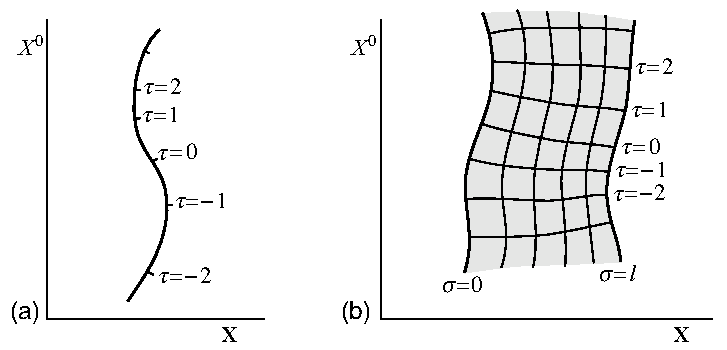
\includegraphics[width=0.8\linewidth]{figures/fig_1_3.pdf}
\caption{(a) パラメータ表示した点粒子の世界線。(b) パラメータ表示した開弦の世界面。}
\label{fig:1.3}
\end{figure}

パラメータ表示に依存しない、最も単純な Poincaré 不変な作用は、世界線に沿う固有時に比例するものであろう。
\begin{equation}
S_{\mathrm{pp}}=-m\int d\tau\,(-\dot X^\mu\dot X_\mu)^{1/2}.
\tag{1.2.2}\label{eq:1.2.2}
\end{equation}
ここで、ドットは $\tau$ に関する微分を表す。部分積分すると、作用の変分は
\begin{equation}
\delta S_{\mathrm{pp}}=-m\int d\tau\,\dot u_\mu\,\delta X^\mu
\tag{1.2.3}\label{eq:1.2.3}
\end{equation}
となる。ただし、
\begin{equation}
u^\mu=\dot X^\mu(-\dot X^\nu\dot X_\nu)^{-1/2}
\tag{1.2.4}\label{eq:1.2.4}
\end{equation}
は規格化された $D$ 元速度である。したがって、運動方程式 $\dot u^\mu=0$ は自由運動を記述する。非相対論的極限を見ることで確認できるように、規格化定数 $m$ は粒子の質量である（演習1.1）。

世界線上に追加の場、すなわち独立な世界線計量 $\gamma_{\tau\tau}(\tau)$ を導入すれば、作用をもう一つの便利な形に書ける。正であると定義したテトラッド $\eta(\tau)=(-\gamma_{\tau\tau}(\tau))^{1/2}$ を用いると便利である。テトラッドという語の語根は「四」を意味するが、ここでは一般相対論のこの用語を任意の次元数で用いる。このとき
\begin{equation}
S'_{\mathrm{pp}}=\frac12\int d\tau\,
\bigl(\eta^{-1}\dot X^\mu\dot X_\mu-\eta m^2\bigr).
\tag{1.2.5}\label{eq:1.2.5}
\end{equation}
この作用は、先ほどの作用 $S_{\mathrm{pp}}$ と同じ対称性、すなわち Poincaré 不変性と世界線の再パラメータ化不変性をもつ。後者の下で $\eta(\tau)$ は
\begin{equation}
\eta'(\tau')\,d\tau'=\eta(\tau)\,d\tau
\tag{1.2.6}\label{eq:1.2.6}
\end{equation}
と変換する。

テトラッドを変分して得られる運動方程式は
\begin{equation}
\eta^2=-\dot X^\mu\dot X_\mu/m^2
\tag{1.2.7}\label{eq:1.2.7}
\end{equation}
である。これを用いて $\eta(\tau)$ を消去すると、作用 $S'_{\mathrm{pp}}$ は先ほどの $S_{\mathrm{pp}}$ となる。ちなみに、$S'_{\mathrm{pp}}$ は質量のない粒子に対してもまったく問題なく意味をもつが、その場合 $S_{\mathrm{pp}}$ は使えない。

作用 $S_{\mathrm{pp}}$ と $S'_{\mathrm{pp}}$ は古典的には等価であるが、$S_{\mathrm{pp}}$ は微分を平方根の内部に含む複雑な形をしているため、経路積分の中で意味を与えることが難しい。一方、$S'_{\mathrm{pp}}$ は微分について二次であり、その経路積分は、後の章で見るように、かなり容易に評価できる。おそらく、$S_{\mathrm{pp}}$ に対して量子論を定義しようとするどのような試みも、$S'_{\mathrm{pp}}$ の経路積分と等価な結果へ至るであろう。そこで、後者を量子論の定義の出発点とする。

一次元の物体は、図\hyperref[fig:1.3]{1.3}(b)のように、二つのパラメータを用いた $X^\mu(\tau,\sigma)$ によって記述できる二次元の世界面を描く。粒子の場合と同様、作用などの物理量は、時空への埋め込みのみに依存し、パラメータ表示には依存しないことを要求する。理論がこの性質をもつことは魅力的であるばかりでなく、整合的な相対論的量子論には必要であることも見るであろう。最も単純な不変作用である Nambu--Goto 作用は、世界面の面積に比例する。この作用を $X^\mu(\tau,\sigma)$ によって表すため、まず誘導計量 $h_{ab}$ を定義する。添字 $a,b,\ldots$ は $(\tau,\sigma)$ の値をとる。
\begin{equation}
h_{ab}=\partial_aX^\mu\partial_bX_\mu.
\tag{1.2.8}\label{eq:1.2.8}
\end{equation}
すると Nambu--Goto 作用は
\begin{align}
S_{\mathrm{NG}}&=\int_M d\tau\,d\sigma\,\mathcal L_{\mathrm{NG}},
\tag{1.2.9a}\label{eq:1.2.9a}\\
\mathcal L_{\mathrm{NG}}&=-\frac{1}{2\pi\alpha'}(-\det h_{ab})^{1/2}
\tag{1.2.9b}\label{eq:1.2.9b}
\end{align}
となる。ここで $M$ は世界面を表す。時空の長さの二乗の単位をもつ定数 $\alpha'$ は Regge 勾配であり、その意味は後で明らかになる。弦の張力 $T$ と Regge 勾配の関係は
\begin{equation}
T=\frac{1}{2\pi\alpha'}
\tag{1.2.10}\label{eq:1.2.10}
\end{equation}
である（演習1.1）。

次に、作用の対称性、すなわち $S_{\mathrm{NG}}[X']=S_{\mathrm{NG}}[X]$ となる $X^\mu(\tau,\sigma)$ の変換を考えよう。これらは次のものである。
\begin{enumerate}
\item 平坦な時空の等長変換群、すなわち $D$ 次元 Poincaré 群：
\begin{equation}
X'^\mu(\tau,\sigma)=\Lambda^\mu{}_\nu X^\nu(\tau,\sigma)+a^\mu.
\tag{1.2.11}\label{eq:1.2.11}
\end{equation}
ここで $\Lambda^\mu{}_\nu$ は Lorentz 変換、$a^\mu$ は並進である。
\item 二次元の座標不変性。しばしば微分同相（diff）不変性と呼ばれる。新しい座標 $(\tau'(\tau,\sigma),\sigma'(\tau,\sigma))$ に対し、変換は
\begin{equation}
X'^\mu(\tau',\sigma')=X^\mu(\tau,\sigma)
\tag{1.2.12}\label{eq:1.2.12}
\end{equation}
である。
\end{enumerate}

Nambu--Goto 作用は、平方根の中に微分を含む点で、点粒子の作用 $S_{\mathrm{pp}}$ に類似している。ここでも、独立な世界面計量 $\gamma_{ab}(\tau,\sigma)$ を導入することによって単純化できる。以下では、「誘導」と明示しない限り、「計量」は常に $\gamma_{ab}$ を意味し、添字の上げ下げも常にこの計量を用いて行う。$\gamma_{ab}$ は Lorentz 型の符号 $(-,+)$ をもつものとする。作用は
\begin{equation}
S_{\mathrm P}[X,\gamma]=-\frac{1}{4\pi\alpha'}
\int_M d\tau\,d\sigma\,(-\gamma)^{1/2}\gamma^{ab}
\partial_aX^\mu\partial_bX_\mu
\tag{1.2.13}\label{eq:1.2.13}
\end{equation}
であり、$\gamma=\det\gamma_{ab}$ である。これは Brink--Di Vecchia--Howe--Deser--Zumino 作用、略して Polyakov 作用である。Brink、Di Vecchia、Howe、および Deser と Zumino が、世界面の局所超対称性をもつ一般化を導く過程で見いだした。その利点、とくに経路積分量子化における利点を強調したのは Polyakov である。

$S_{\mathrm{NG}}$ との等価性を見るため、計量を変分して得られる運動方程式を用いる。
\begin{equation}
\delta_\gamma S_{\mathrm P}[X,\gamma]=-\frac{1}{4\pi\alpha'}
\int_M d\tau\,d\sigma\,(-\gamma)^{1/2}\delta\gamma^{ab}
\left(h_{ab}-\frac12\gamma_{ab}\gamma^{cd}h_{cd}\right).
\tag{1.2.14}\label{eq:1.2.14}
\end{equation}
ここで $h_{ab}$ は、やはり誘導計量\hyperref[eq:1.2.8]{(1.2.8)}である。行列式の変分に関する一般的な関係
\begin{equation}
\delta\gamma=\gamma\gamma^{ab}\delta\gamma_{ab}
=-\gamma\gamma_{ab}\delta\gamma^{ab}
\tag{1.2.15}\label{eq:1.2.15}
\end{equation}
を用いた。すると、$\delta_\gamma S_{\mathrm P}=0$ は
\begin{equation}
h_{ab}=\frac12\gamma_{ab}\gamma^{cd}h_{cd}
\tag{1.2.16}\label{eq:1.2.16}
\end{equation}
を意味する。この方程式を、その行列式にマイナスを付けたものの平方根で割ると、
\begin{equation}
h_{ab}(-h)^{-1/2}=\gamma_{ab}(-\gamma)^{-1/2}
\tag{1.2.17}\label{eq:1.2.17}
\end{equation}
が得られる。したがって、$\gamma_{ab}$ は誘導計量に比例する。さらにこれを用いて、作用から $\gamma_{ab}$ を消去できる。
\begin{equation}
S_{\mathrm P}[X,\gamma]\longrightarrow
-\frac{1}{2\pi\alpha'}\int d\tau\,d\sigma\,(-h)^{1/2}
=S_{\mathrm{NG}}[X].
\tag{1.2.18}\label{eq:1.2.18}
\end{equation}

作用 $S_{\mathrm P}$ は、次の対称性をもつ。
\begin{enumerate}
\item $D$ 次元 Poincaré 不変性：
\begin{equation}
\begin{aligned}
X'^\mu(\tau,\sigma)&=\Lambda^\mu{}_\nu X^\nu(\tau,\sigma)+a^\mu,\\
\gamma'_{ab}(\tau,\sigma)&=\gamma_{ab}(\tau,\sigma).
\end{aligned}
\tag{1.2.19}\label{eq:1.2.19}
\end{equation}
\item 微分同相不変性：
\begin{equation}
\begin{aligned}
X'^\mu(\tau',\sigma')&=X^\mu(\tau,\sigma),\\
\frac{\partial\sigma'^c}{\partial\sigma^a}
\frac{\partial\sigma'^d}{\partial\sigma^b}\gamma'_{cd}(\tau',\sigma')
&=\gamma_{ab}(\tau,\sigma),
\end{aligned}
\tag{1.2.20}\label{eq:1.2.20}
\end{equation}
ここで $\sigma'^a(\tau,\sigma)$ は新しい座標である。
\item 二次元 Weyl 不変性：
\begin{equation}
\begin{aligned}
X'^\mu(\tau,\sigma)&=X^\mu(\tau,\sigma),\\
\gamma'_{ab}(\tau,\sigma)&=\exp\bigl(2\omega(\tau,\sigma)\bigr)
\gamma_{ab}(\tau,\sigma),
\end{aligned}
\tag{1.2.21}\label{eq:1.2.21}
\end{equation}
ここで $\omega(\tau,\sigma)$ は任意である。
\end{enumerate}
世界面計量の局所的なスケール変換である Weyl 不変性に相当するものは、Nambu--Goto の形式にはない。それが現れる理由は、Polyakov 作用と Nambu--Goto 作用を結びつけるのに用いた運動方程式\hyperref[eq:1.2.17]{(1.2.17)}を振り返ることで理解できる。この式は $\gamma_{ab}$ を完全には決めず、局所的なスケール変換の自由度を残してしか決めない。そのため、Weyl 変換で等価な計量は、時空への同じ埋め込みに対応する。これは、明らかな微分同相不変性に加えて、Polyakov の定式化がもつ追加の冗長性である。

計量に関する作用の変分によって、エネルギー運動量テンソルを定義する。
\begin{equation}
\begin{aligned}
T^{ab}(\tau,\sigma)&=-4\pi(-\gamma)^{-1/2}
\frac{\delta}{\delta\gamma_{ab}}S_{\mathrm P}\\
&=-\frac{1}{\alpha'}\left(
\partial^aX^\mu\partial^bX_\mu
-\frac12\gamma^{ab}\partial_cX^\mu\partial^cX_\mu\right).
\end{aligned}
\tag{1.2.22}\label{eq:1.2.22}
\end{equation}
これは、場の理論における通常の定義に比べて $-2\pi$ という余分な因子をもつ。弦理論では、これが標準的で便利な規約である。微分同相不変性の帰結として、これは保存する：$\nabla_aT^{ab}=0$。さらに、任意の Weyl 変換に対する $S_{\mathrm P}$ の不変性は、
\begin{equation}
\gamma_{ab}\frac{\delta}{\delta\gamma_{ab}}S_{\mathrm P}=0
\quad\Rightarrow\quad T^a{}_a=0
\tag{1.2.23}\label{eq:1.2.23}
\end{equation}
を意味する。

作用 $S_{\mathrm{NG}}$ と $S_{\mathrm P}$ は、弦の世界面上の二次元場の理論を定義する。弦理論では、時空内の過程の振幅が、世界面上の二次元場の量子論における行列要素によって与えられることを見るであろう。われわれの関心は四次元時空にあるが、弦の摂動論で用いる道具の大部分は二次元のものである。世界面の観点では、座標変換則\hyperref[eq:1.2.12]{(1.2.12)}は $X^\mu(\tau,\sigma)$ をスカラー場と定義しており、$\mu$ は内部添字として付随している。二次元の観点からは、Polyakov 作用は計量 $\gamma_{ab}$ に共変的に結合した、質量のない Klein--Gordon スカラー $X^\mu$ を記述する。また、この観点では Poincaré 不変性は内部対称性である。すなわち、$\tau,\sigma$ を固定した場に作用する。

作用で $\gamma_{ab}$ を変分すると、運動方程式
\begin{equation}
T_{ab}=0
\tag{1.2.24}\label{eq:1.2.24}
\end{equation}
が得られる。$X^\mu$ を変分すると、運動方程式
\begin{equation}
\partial_a\bigl[(-\gamma)^{1/2}\gamma^{ab}\partial_bX^\mu\bigr]
=(-\gamma)^{1/2}\nabla^2X^\mu=0
\tag{1.2.25}\label{eq:1.2.25}
\end{equation}
が得られる。境界をもつ世界面では、作用の変分に表面項も現れる。具体的に、座標領域を
\begin{equation}
-\infty<\tau<\infty,\qquad 0\leq\sigma\leq\ell
\tag{1.2.26}\label{eq:1.2.26}
\end{equation}
としよう。$\tau$ を時間変数、$\sigma$ を空間的な変数と考えるので、これは源なしで伝播する一本の弦である。このとき
\begin{equation}
\begin{aligned}
\delta S_{\mathrm P}
={}&\frac{1}{2\pi\alpha'}\int_{-\infty}^{\infty}d\tau
\int_0^\ell d\sigma\,(-\gamma)^{1/2}\delta X^\mu\nabla^2X_\mu\\
&-\frac{1}{2\pi\alpha'}\int_{-\infty}^{\infty}d\tau\,
\left.(-\gamma)^{1/2}\delta X^\mu\partial^\sigma X_\mu
\right|_{\sigma=0}^{\sigma=\ell}.
\end{aligned}
\tag{1.2.27}\label{eq:1.2.27}
\end{equation}
内部では、運動方程式は先ほどと同じである。
\begin{equation}
\partial^\sigma X^\mu(\tau,0)=\partial^\sigma X^\mu(\tau,\ell)=0
\tag{1.2.28}\label{eq:1.2.28}
\end{equation}
ならば、境界項は消える。これらは $X^\mu$ に対する Neumann 境界条件である。より共変的に述べると、
\begin{equation}
n^a\partial_aX_\mu=0\qquad \text{$\partial M$ 上で}
\tag{1.2.29}\label{eq:1.2.29}
\end{equation}
となる。ここで $n^a$ は境界 $\partial M$ に垂直である。開弦の両端は、時空内を自由に動く。

また、
\begin{align}
X^\mu(\tau,\ell)&=X^\mu(\tau,0),&
\partial^\sigma X^\mu(\tau,\ell)&=\partial^\sigma X^\mu(\tau,0),
\tag{1.2.30a}\label{eq:1.2.30a}\\
\gamma_{ab}(\tau,\ell)&=\gamma_{ab}(\tau,0)
\tag{1.2.30b}\label{eq:1.2.30b}
\end{align}
を課しても、運動方程式の表面項は消える。つまり、場は周期的である。境界は存在せず、両端は結び合わされて閉じた輪をなす。

開弦の境界条件\hyperref[eq:1.2.28]{(1.2.28)}と閉弦の境界条件\hyperref[eq:1.2.30a]{(1.2.30)}が、$D$ 次元 Poincaré 不変性および運動方程式と両立する唯一の可能性である。Poincaré 不変性の条件を緩めると、ほかの可能性もあり、後に重要になる。その一部は演習で調べる。

Nambu--Goto 作用と Polyakov 作用は、与えられた対称性をもつ最も単純な作用かもしれない。しかし、作用の単純さは、場の量子論における正しい基準ではない。鍵となる考えは、単純さではなく対称性である。物理的理由と技術的理由の両方から、通常は理論のすべての対称性と両立する最も一般的な局所作用を考えねばならない。対称性が保たれ、作用が微分の多項式であることを要求して、Polyakov 作用を一般化してみよう（そうでなければ量子論に意味を与えることが難しい）。\footnote[3]{この要請を緩めると、誘導計量 $h_{ab}$ の曲率から構成される不変量など、さまざまな追加の可能性が生じる。電束管や磁束管のような一次元の物体では、そのような項が現れると予想され、その場合は物体の太さがカットオフを与えるため、経路積分は意味をもつ。しかし、基礎的な弦理論で扱うような、無限に細い弦ではこれは不可能である。}
大域的な Weyl 不変性、すなわち $\omega(\tau,\sigma)=\text{定数}$ は、$(-\gamma)^{1/2}$ の変化を打ち消すために、作用において $\gamma^{ab}$ の因子の数が $\gamma_{ab}$ の因子の数より一つ多いことを要求する。余った上付き添字は微分としか縮約できないため、各項は正確に二つの微分を含む。すると、座標不変性と Poincaré 不変性から、元の $S_{\mathrm P}$ に加えて、次の一つの項が許される。
\begin{equation}
\chi=\frac{1}{4\pi}\int_M d\tau\,d\sigma\,(-\gamma)^{1/2}R.
\tag{1.2.31}\label{eq:1.2.31}
\end{equation}
ここで $R$ は、$\gamma_{ab}$ から構成される Ricci スカラーである。局所的な Weyl スケール変換の下で、
\begin{equation}
(-\gamma')^{1/2}R'=(-\gamma)^{1/2}\bigl(R-2\nabla^2\omega\bigr).
\tag{1.2.32}\label{eq:1.2.32}
\end{equation}
任意の $v^a$ に対し $(-\gamma)^{1/2}\nabla_av^a
=\partial_a\bigl((-\gamma)^{1/2}v^a\bigr)$ であるため、この変分は全微分である。したがって積分\hyperref[eq:1.2.31]{(1.2.31)}は、境界をもたない世界面では不変である。境界がある場合には、追加の表面項が必要となる（演習1.3）。

$\chi$ は対称性によって許されるので、作用に含めることにする。
\begin{equation}
\begin{aligned}
S'_{\mathrm P}&=S_{\mathrm P}-\lambda\chi\\
&=-\int_M d\tau\,d\sigma\,(-\gamma)^{1/2}
\left(\frac{1}{4\pi\alpha'}\gamma^{ab}\partial_aX^\mu\partial_bX_\mu
+\frac{\lambda}{4\pi}R\right).
\end{aligned}
\tag{1.2.33}\label{eq:1.2.33}
\end{equation}
これは、これらの場と対称性のもとで、$(\text{diff}\times\text{Weyl})$ 不変かつ Poincaré 不変な最も一般的な作用である。当面、対称性についての議論は古典的なものであり、量子異常の可能性は無視している。それについては第3章で考察する。

作用 $S'_{\mathrm P}$ は、計量に対する Hilbert 作用 $\int(-\gamma)^{1/2}R$ に、$D$ 個の質量のないスカラー場 $X^\mu$ を最小結合したものに見える。しかし二次元では、Hilbert 作用は世界面の位相のみに依存し、計量に力学を与えない。このことを見るため、その変分が $R_{ab}-\tfrac12\gamma_{ab}R$ に比例するという一般相対論の結果を用いる。二次元では、曲率テンソルの対称性から $R_{ab}=\tfrac12\gamma_{ab}R$ が従うため、これはゼロになる。すなわち、Hilbert 作用は計量の任意の連続変化に対して不変である。ただし、第3章で見るように、何らかの大域的な意味はもっている。

理論をさらに一般化しようとする方法はいろいろある。一つは、最終的な関心が $D=4$ にあることに示唆されるもので、$X^\mu$ 場を四つより多く許しつつ、四次元 Poincaré 不変性だけを要求するというものである。第二は、対称性こそが最も重要であるという考えに動機づけられるもので、同じ局所対称性と四次元 Poincaré 不変性を保ちつつ、より一般的な場の内容を許すというものである。すなわち、世界面および時空の対称群の異なる表現に属する二次元の場を許す。これらの考えはいずれも重要であり、さまざまな機会に立ち戻ることになる。さらに別の考えは、理論の局所対称性を拡大することであり、第2巻ではこの考えを追求する。
